\documentclass[tikz,border=14pt]{standalone}
\usepackage{xcolor}
\usetikzlibrary{
    positioning,
    arrows.meta,
    shapes.geometric,
    fit,
    backgrounds,
    calc,
    shadows.blur,
    fadings,
    decorations.pathreplacing
}
\usepackage{helvet}
\renewcommand{\familydefault}{\sfdefault}

% -------------------------------------------------
% ELEGANT JOURNAL PALETTE (muted, print-safe)
% -------------------------------------------------
\definecolor{mainborder}{RGB}{31,78,121}
\definecolor{mainfill}{RGB}{236,244,252}
\definecolor{mainglow}{RGB}{200,220,240}

\definecolor{stepborder}{RGB}{22,110,102}
\definecolor{stepfill}{RGB}{230,246,243}
\definecolor{stepglow}{RGB}{190,225,220}

\definecolor{analborder}{RGB}{92,58,142}
\definecolor{analfill}{RGB}{242,237,251}
\definecolor{analglow}{RGB}{215,200,235}

\definecolor{exclborder}{RGB}{176,42,55}
\definecolor{exclfill}{RGB}{252,236,238}
\definecolor{exclglow}{RGB}{240,200,205}

\definecolor{numfill}{RGB}{255,246,228}
\definecolor{numborder}{RGB}{200,130,30}
\definecolor{numglow}{RGB}{250,220,170}

\definecolor{sensborder}{RGB}{35,120,75}
\definecolor{sensfill}{RGB}{232,247,238}
\definecolor{sensglow}{RGB}{190,225,205}

\definecolor{framegray}{RGB}{165,172,185}
\definecolor{softgray}{RGB}{130,138,152}
\definecolor{deepnavy}{RGB}{20,45,75}

\begin{document}
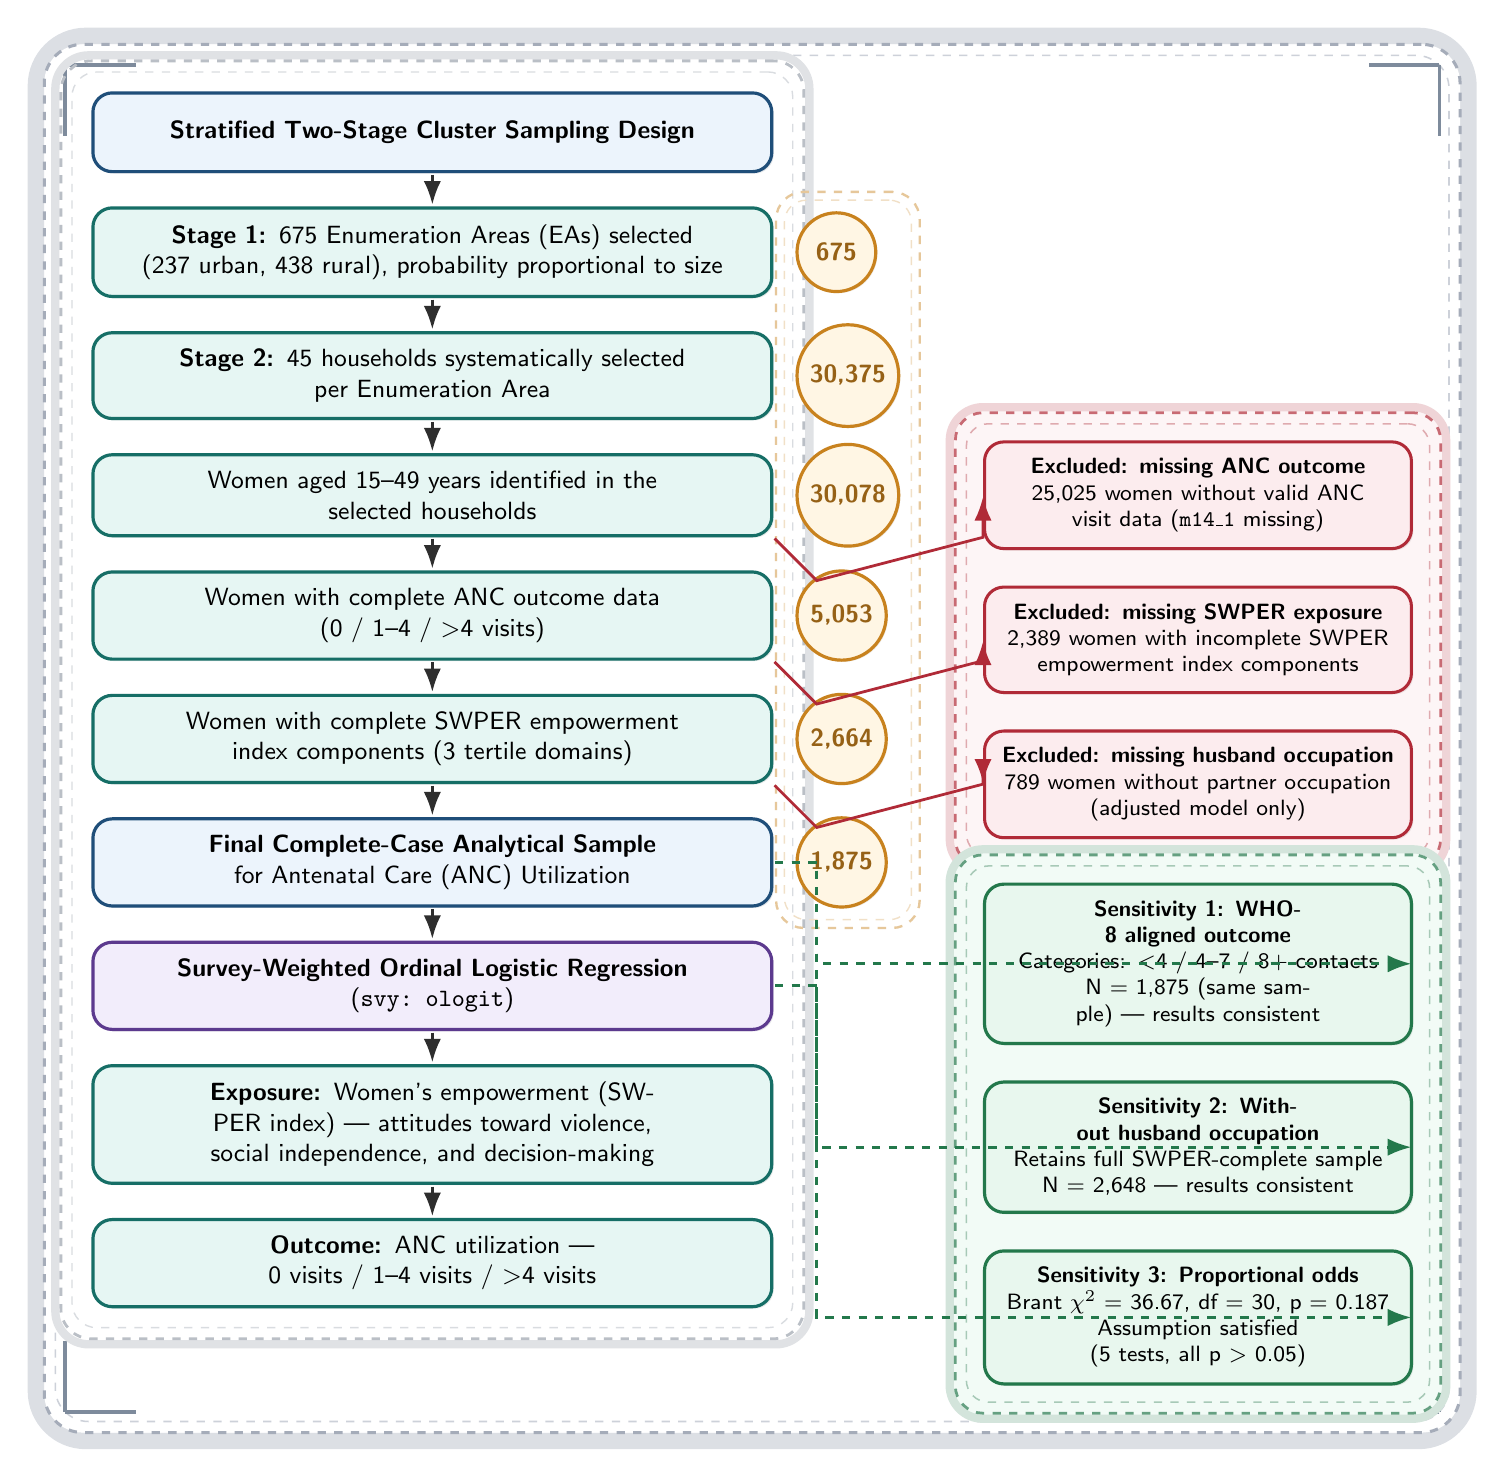
\begin{tikzpicture}[
    node distance=0.42cm and 1.35cm,
    font=\sffamily\small,
    % ---------- MAIN SPINE BOXES ----------
    mainbox/.style={
        rectangle, rounded corners=7pt,
        draw=mainborder, fill=mainfill, line width=1.15pt,
        align=center, text width=8.2cm,
        minimum height=1.00cm, inner sep=6pt,
        drop shadow={shadow xshift=0.7pt, shadow yshift=-0.7pt,
                     opacity=0.25, fill=mainglow!70!black}
    },
    stepbox/.style={
        rectangle, rounded corners=7pt,
        draw=stepborder, fill=stepfill, line width=1.15pt,
        align=center, text width=8.2cm,
        minimum height=1.00cm, inner sep=6pt,
        drop shadow={shadow xshift=0.7pt, shadow yshift=-0.7pt,
                     opacity=0.22, fill=stepglow!70!black}
    },
    analysisbox/.style={
        rectangle, rounded corners=7pt,
        draw=analborder, fill=analfill, line width=1.15pt,
        align=center, text width=8.2cm,
        minimum height=1.00cm, inner sep=6pt,
        drop shadow={shadow xshift=0.7pt, shadow yshift=-0.7pt,
                     opacity=0.25, fill=analglow!70!black}
    },
    % ---------- EXCLUSION BOXES ----------
    exclbox/.style={
        rectangle, rounded corners=7pt,
        draw=exclborder, fill=exclfill, line width=1.1pt,
        align=center, text width=5.0cm,
        minimum height=1.00cm, inner sep=6pt,
        font=\sffamily\footnotesize,
        drop shadow={shadow xshift=0.7pt, shadow yshift=-0.7pt,
                     opacity=0.20, fill=exclglow!70!black}
    },
    % ---------- SENSITIVITY BOXES ----------
    sensbox/.style={
        rectangle, rounded corners=7pt,
        draw=sensborder, fill=sensfill, line width=1.15pt,
        align=center, text width=5.0cm,
        minimum height=1.00cm, inner sep=6pt,
        font=\sffamily\footnotesize,
        drop shadow={shadow xshift=0.7pt, shadow yshift=-0.7pt,
                     opacity=0.22, fill=sensglow!70!black}
    },
    % ---------- SAMPLE COUNT CIRCLES ----------
    samplenum/.style={
        circle, minimum size=1.00cm,
        draw=numborder, fill=numfill, line width=1.15pt,
        font=\sffamily\small\bfseries,
        text=numborder!75!black,
        drop shadow={shadow xshift=0.6pt, shadow yshift=-0.6pt,
                     opacity=0.22, fill=numglow!70!black}
    },
    % ---------- ARROWS ----------
    flowarrow/.style={
        -{Latex[length=3.0mm,width=2.2mm]},
        line width=1.05pt, draw=black!82,
        shorten >=0.6pt, shorten <=0.6pt
    },
    exclarrow/.style={
        -{Latex[length=3.0mm,width=2.2mm]},
        line width=1.0pt, draw=exclborder,
        shorten >=0.6pt, shorten <=0.6pt
    },
    sensarrow/.style={
        -{Latex[length=3.0mm,width=2.2mm]},
        line width=1.0pt, draw=sensborder,
        shorten >=0.6pt, shorten <=0.6pt
    }
]

% ============================================================
% LAYER 1 (LEFT COLUMN) — MAIN ANALYSIS SPINE
% ============================================================
\node[mainbox] (title)
    {\textbf{Stratified Two-Stage Cluster Sampling Design}};

\node[stepbox, below=of title] (stage1)
    {\textbf{Stage 1:} 675 Enumeration Areas (EAs) selected\\
     (237 urban, 438 rural), probability proportional to size};

\node[stepbox, below=of stage1] (stage2)
    {\textbf{Stage 2:} 45 households systematically selected\\
     per Enumeration Area};

\node[stepbox, below=of stage2] (women)
    {Women aged 15--49 years identified in the\\
     selected households};

\node[stepbox, below=of women] (ancavail)
    {Women with complete ANC outcome data\\
     (0 / 1--4 / $>$4 visits)};

\node[stepbox, below=of ancavail] (swpercomp)
    {Women with complete SWPER empowerment\\
     index components (3 tertile domains)};

\node[mainbox, below=of swpercomp] (final)
    {\textbf{Final Complete-Case Analytical Sample}\\
     for Antenatal Care (ANC) Utilization};

\node[analysisbox, below=of final] (analysis)
    {\textbf{Survey-Weighted Ordinal Logistic Regression}\\
     (\texttt{svy: ologit})};

\node[stepbox, below=of analysis] (exposure)
    {\textbf{Exposure:} Women's empowerment (SWPER index) ---
     attitudes toward violence, social independence,
     and decision-making};

\node[stepbox, below=of exposure] (outcome)
    {\textbf{Outcome:} ANC utilization ---
     0 visits / 1--4 visits / $>$4 visits};

% ============================================================
% MIDDLE COLUMN — SAMPLE COUNT CIRCLES
% ============================================================
\node[samplenum, right=0.28cm of stage1]    (n1) {675};
\node[samplenum, right=0.28cm of stage2]    (n2) {30{,}375};
\node[samplenum, right=0.28cm of women]     (n3) {30{,}078};
\node[samplenum, right=0.28cm of ancavail]  (n4) {5{,}053};
\node[samplenum, right=0.28cm of swpercomp] (n5) {2{,}664};
\node[samplenum, right=0.28cm of final]     (n6) {1{,}875};

% ============================================================
% LAYER 2 (RIGHT COLUMN) — EXCLUSIONS + SENSITIVITY ANALYSES
% ============================================================

% --- EXCLUSION 1: Missing ANC ---
\node[exclbox, right=1.05cm of n3] (missing_anc)
    {\textbf{Excluded: missing ANC outcome}\\
     25{,}025 women without valid ANC\\
     visit data (\texttt{m14\_1} missing)};

% --- EXCLUSION 2: Missing SWPER ---
\node[exclbox, below=0.45cm of missing_anc] (missing_swper)
    {\textbf{Excluded: missing SWPER exposure}\\
     2{,}389 women with incomplete SWPER\\
     empowerment index components};

% --- EXCLUSION 3: Missing husband occupation ---
\node[exclbox, below=0.45cm of missing_swper] (missing_husbocc)
    {\textbf{Excluded: missing husband occupation}\\
     789 women without partner occupation\\
     (adjusted model only)};

% --- SENSITIVITY 1: WHO-8 aligned ---
\node[sensbox, below=0.55cm of missing_husbocc] (sens_who)
    {\textbf{Sensitivity 1: WHO-8 aligned outcome}\\
     Categories: $<$4 / 4--7 / 8+ contacts\\
     N = 1{,}875 (same sample) --- results consistent};

% --- SENSITIVITY 2: Without husband occupation ---
\node[sensbox, below=0.45cm of sens_who] (sens_husbocc)
    {\textbf{Sensitivity 2: Without husband occupation}\\
     Retains full SWPER-complete sample\\
     N = 2{,}648 --- results consistent};

% --- SENSITIVITY 3: Proportional odds test ---
\node[sensbox, below=0.45cm of sens_husbocc] (sens_brant)
    {\textbf{Sensitivity 3: Proportional odds}\\
     Brant $\chi^2$ = 36.67, df = 30, p = 0.187\\
     Assumption satisfied (5 tests, all p $>$ 0.05)};

% ============================================================
% FLOW ARROWS — MAIN SPINE
% ============================================================
\draw[flowarrow] (title)     -- (stage1);
\draw[flowarrow] (stage1)    -- (stage2);
\draw[flowarrow] (stage2)    -- (women);
\draw[flowarrow] (women)     -- (ancavail);
\draw[flowarrow] (ancavail)  -- (swpercomp);
\draw[flowarrow] (swpercomp) -- (final);
\draw[flowarrow] (final)     -- (analysis);
\draw[flowarrow] (analysis)  -- (exposure);
\draw[flowarrow] (exposure)  -- (outcome);

% ============================================================
% EXCLUSION ARROWS — ORTHOGONAL (down → right)
% ============================================================
\draw[exclarrow]
    (women.south east) -- ++(0.55,-0.55)
    -- (missing_anc.west |- women.south east)
    -- (missing_anc.west);

\draw[exclarrow]
    (ancavail.south east) -- ++(0.55,-0.55)
    -- (missing_swper.west |- ancavail.south east)
    -- (missing_swper.west);

\draw[exclarrow]
    (swpercomp.south east) -- ++(0.55,-0.55)
    -- (missing_husbocc.west |- swpercomp.south east)
    -- (missing_husbocc.west);

% ============================================================
% SENSITIVITY ARROWS — dashed, from final/analysis to sens boxes
% ============================================================
% From `final` down and right into Sensitivity 1
\draw[sensarrow, dashed]
    (final.east) -- ++(0.55,0)
    |- (sens_who.east);

% From `final` down to Sensitivity 2
\draw[sensarrow, dashed]
    (final.east) -- ++(0.55,0)
    |- (sens_husbocc.east);

% From `analysis` down to Sensitivity 3
\draw[sensarrow, dashed]
    (analysis.east) -- ++(0.55,0)
    |- (sens_brant.east);

% ============================================================
% BACKGROUND LAYER — ELEGANT STYLISH FRAMES
% ============================================================
\begin{scope}[on background layer]

    % ---------- 1. OUTER GLOW ----------
    \node[
        fit=(title)(stage1)(stage2)(women)(ancavail)(swpercomp)(final)
            (analysis)(exposure)(outcome)
            (missing_anc)(missing_swper)(missing_husbocc)
            (sens_who)(sens_husbocc)(sens_brant),
        draw=deepnavy!15, line width=6pt,
        rounded corners=18pt,
        inner sep=20pt
    ] (glow) {};

    % ---------- 2. OUTER DOUBLE DASHED FRAME ----------
    \node[
        fit=(title)(stage1)(stage2)(women)(ancavail)(swpercomp)(final)
            (analysis)(exposure)(outcome)
            (missing_anc)(missing_swper)(missing_husbocc)
            (sens_who)(sens_husbocc)(sens_brant),
        draw=framegray, dashed, line width=1.1pt,
        rounded corners=14pt,
        inner sep=17pt,
        fill=white
    ] (outerframe) {};

    \node[
        fit=(title)(stage1)(stage2)(women)(ancavail)(swpercomp)(final)
            (analysis)(exposure)(outcome)
            (missing_anc)(missing_swper)(missing_husbocc)
            (sens_who)(sens_husbocc)(sens_brant),
        draw=framegray!55, dashed, line width=0.55pt,
        rounded corners=12pt,
        inner sep=13pt
    ] (innerframe) {};

    % ---------- 3. CORNER ACCENTS ----------
    \draw[deepnavy!55, line width=1.4pt, rounded corners=3pt]
        ([xshift=8pt,yshift=-8pt]outerframe.north west) -- ++(0.9cm,0);
    \draw[deepnavy!55, line width=1.4pt, rounded corners=3pt]
        ([xshift=8pt,yshift=-8pt]outerframe.north west) -- ++(0,-0.9cm);

    \draw[deepnavy!55, line width=1.4pt, rounded corners=3pt]
        ([xshift=-8pt,yshift=-8pt]outerframe.north east) -- ++(-0.9cm,0);
    \draw[deepnavy!55, line width=1.4pt, rounded corners=3pt]
        ([xshift=-8pt,yshift=-8pt]outerframe.north east) -- ++(0,-0.9cm);

    \draw[deepnavy!55, line width=1.4pt, rounded corners=3pt]
        ([xshift=8pt,yshift=8pt]outerframe.south west) -- ++(0.9cm,0);
    \draw[deepnavy!55, line width=1.4pt, rounded corners=3pt]
        ([xshift=8pt,yshift=8pt]outerframe.south west) -- ++(0,0.9cm);

    \draw[deepnavy!55, line width=1.4pt, rounded corners=3pt]
        ([xshift=-8pt,yshift=8pt]outerframe.south east) -- ++(-0.9cm,0);
    \draw[deepnavy!55, line width=1.4pt, rounded corners=3pt]
        ([xshift=-8pt,yshift=8pt]outerframe.south east) -- ++(0,0.9cm);

    % ---------- 4. MAIN SPINE SOFT GLOW + DASHED FRAMES ----------
    \node[
        fit=(title)(stage1)(stage2)(women)(ancavail)(swpercomp)(final)
            (analysis)(exposure)(outcome),
        draw=softgray!25, line width=3pt,
        rounded corners=12pt,
        inner sep=13pt
    ] (mainshine) {};

    \node[
        fit=(title)(stage1)(stage2)(women)(ancavail)(swpercomp)(final)
            (analysis)(exposure)(outcome),
        draw=softgray!55, dashed, line width=1.0pt,
        rounded corners=11pt,
        inner sep=11pt
    ] (mainflow) {};

    \node[
        fit=(title)(stage1)(stage2)(women)(ancavail)(swpercomp)(final)
            (analysis)(exposure)(outcome),
        draw=softgray!30, dashed, line width=0.5pt,
        rounded corners=9pt,
        inner sep=7pt
    ] (mainflow2) {};

    % ---------- 5. EXCLUSION CLUSTER GLOW + DASHED FRAMES ----------
    \node[
        fit=(missing_anc)(missing_swper)(missing_husbocc),
        draw=exclborder!20, line width=3pt,
        rounded corners=12pt,
        inner sep=12pt,
        fill=exclfill!55
    ] (exclshine) {};

    \node[
        fit=(missing_anc)(missing_swper)(missing_husbocc),
        draw=exclborder!70, dashed, line width=1.0pt,
        rounded corners=10pt,
        inner sep=10pt
    ] (exclgroup) {};

    \node[
        fit=(missing_anc)(missing_swper)(missing_husbocc),
        draw=exclborder!40, dashed, line width=0.55pt,
        rounded corners=8pt,
        inner sep=6pt
    ] (exclgroup2) {};

    % ---------- 6. SENSITIVITY CLUSTER GLOW + DASHED FRAMES ----------
    \node[
        fit=(sens_who)(sens_husbocc)(sens_brant),
        draw=sensborder!20, line width=3pt,
        rounded corners=12pt,
        inner sep=12pt,
        fill=sensfill!55
    ] (sensshine) {};

    \node[
        fit=(sens_who)(sens_husbocc)(sens_brant),
        draw=sensborder!70, dashed, line width=1.0pt,
        rounded corners=10pt,
        inner sep=10pt
    ] (sensgroup) {};

    \node[
        fit=(sens_who)(sens_husbocc)(sens_brant),
        draw=sensborder!40, dashed, line width=0.55pt,
        rounded corners=8pt,
        inner sep=6pt
    ] (sensgroup2) {};

    % ---------- 7. SAMPLE-CIRCLE BAND ----------
    \node[
        fit=(n1)(n2)(n3)(n4)(n5)(n6),
        draw=numborder!45, dashed, line width=0.85pt,
        rounded corners=10pt,
        inner sep=7pt
    ] (numgroup) {};

    \node[
        fit=(n1)(n2)(n3)(n4)(n5)(n6),
        draw=numborder!25, dashed, line width=0.5pt,
        rounded corners=8pt,
        inner sep=4pt
    ] (numgroup2) {};

\end{scope}

\end{tikzpicture}
\end{document}